%!TEX root = ../../../adrien_gomar_phd.tex

% \subsection{Static aeroelasticity}
% \label{sub:static_aeroelasticity}

% Under some steady centrifugal and gas loads, 
% the blades deform as the structure is elastic.
% However, this deformation is not taken into account while
% designing the blade. Therefore, the shape of the blade is
% not optimum and a loss of efficiency is to be expect.
% From an engineering standpoint, the problem is thus inverse:
% what should be the rigid design of a blade so that under 
% the different loads, it is optimum?

% According to \citet{Marshall1996}, the stiffness of the
% materials used in turbomachinery is large enough to
% prevent from static aeroelasticity. 

\subsection{Flutter}
\label{sub:flutter}

Flutter in turbomachinery is defined as a self-excited, unstable 
self-sustained vibration of a blade. One of the most impressive
manifestation of flutter occurred November 7\textsuperscript{th}, 1940.
\begin{figure}[htb]
  \centering
  \subfigure[Torsion mode]{
      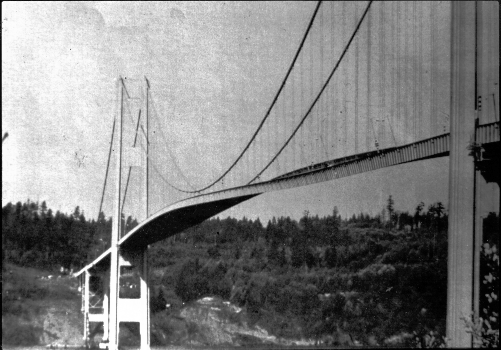
\includegraphics[height=.3\textwidth]{tac06.png}}
  \subfigure[Failure of the bridge]{
      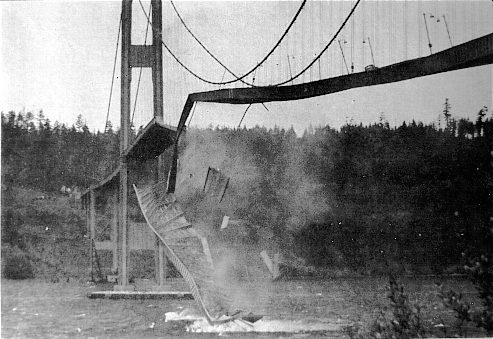
\includegraphics[height=.3\textwidth]{tac09.png}}
  \caption{Tacoma Narrows bridge flutter, from \citet{Smith1974}.}
  \label{fig:tacoma_bridge}
\end{figure}
Four month after being build, the bridge experienced 
torsional flutter excited by a $64$ \mbox{km/h} wind.
A few hours latter the bridge felt down as seen in 
Fig.~\ref{fig:tacoma_bridge}. Hopefully, no human
was injured, but this event showed the importance
of taking into account the flutter phenomenon.

Three vibration scenarios can appear for turbomachinery flutter.
The first scenario is the damped (or positively damped) 
vibration meaning
that the vibration amplitude decreases with respect to time, 
as shown in Fig.~\ref{fig:flutter_damped}.
This is the wished behavior. In this case, the blade is said to
be flutter-free.
The second scenario is the amplified (or negatively damped)
vibration as shown in Fig.~\ref{fig:flutter_amplified}. 
This was the scenario that most likely occurred for the
previous example of the Tacoma bridge. This scenario ultimately
leads to failure which is not acceptable. Furthermore, as
detailed in Sec.~\ref{sec:cror_challenges}, the blades of 
a CROR shall not fail otherwise the aircraft might
be destroyed.
The last scenario is the Limit Cycle Oscillation (LCO) vibration.
In this scenario, the deformation increases until a certain 
amplitude and then stays constant. This scenario is not
destructive by essence compared to the amplified scenario. However,
if the blade is repetitively excited by LCO, the blade
can fail as a consequence of the fatigue of the structure.
\begin{figure}[htb]
  \centering
  \subfigure[damped]{
      \label{fig:flutter_damped}
      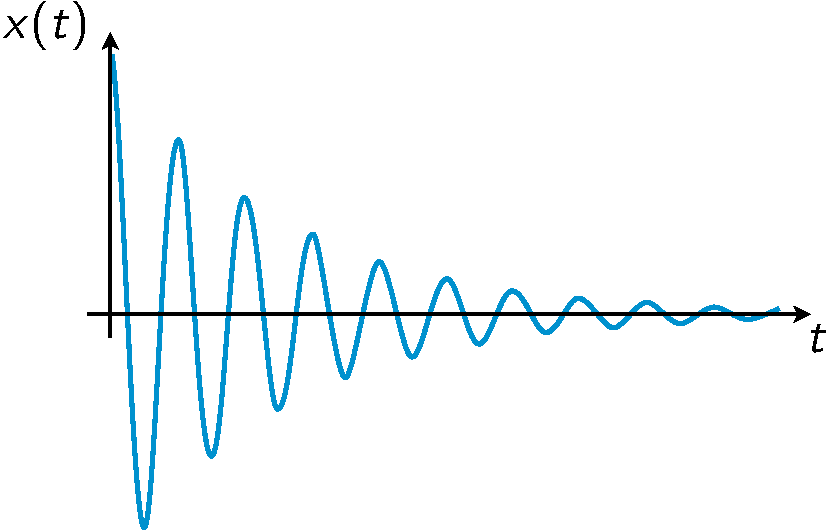
\includegraphics[width=.3\textwidth]{flutter_damped.pdf}}
  \subfigure[amplified]{
      \label{fig:flutter_amplified}
      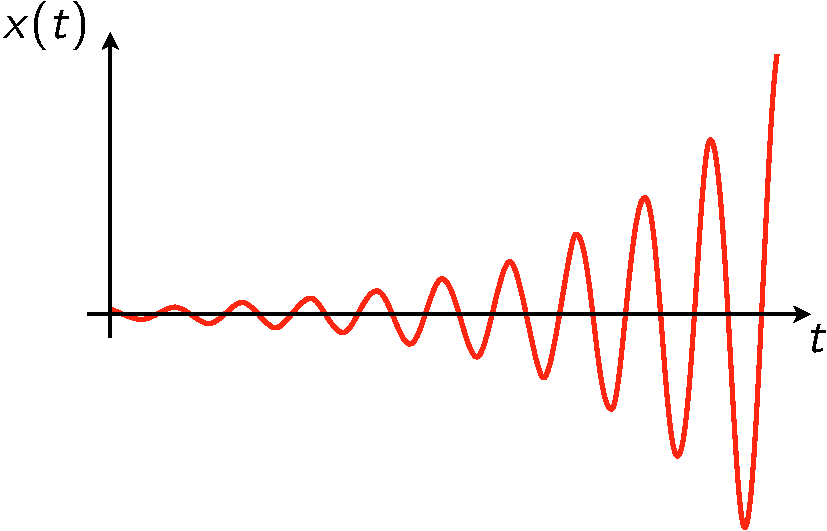
\includegraphics[width=.3\textwidth]{flutter_amplified.pdf}}
  \subfigure[Limit cycle oscillation]{
      \label{fig:LCO}
      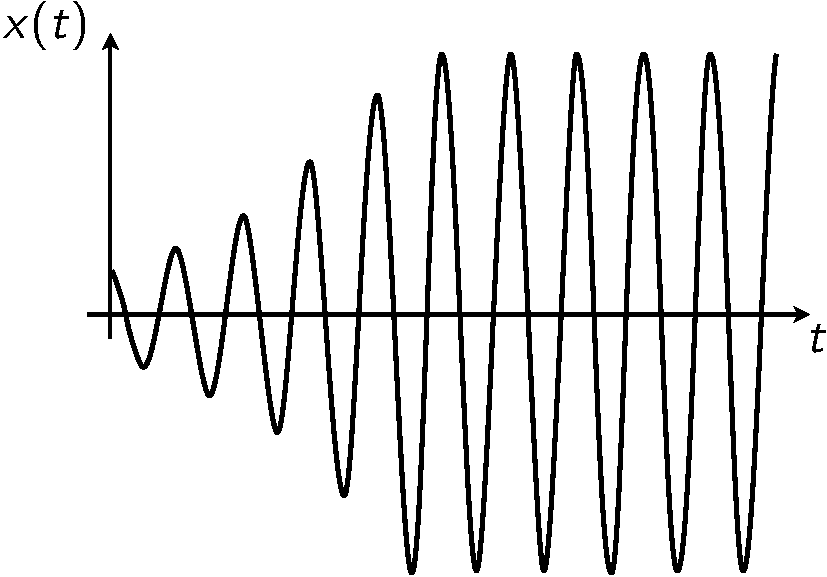
\includegraphics[width=.3\textwidth]{LCO.pdf}}
  \caption{Different vibration scenario for the flutter phenomenon.}
\end{figure}



